\documentclass[
  captions=tableheading,
  bibliography=totoc, 
  titepage=firstiscover,
]{scrartcl}

\usepackage{blindtext} %neuer input

\usepackage{longtable} % Tabellen über mehrere Seiten

\usepackage[utf8]{inputenc} %neuer input

\usepackage{scrhack}

\usepackage[aux]{rerunfilecheck} %Warnung falls nochmal kompiliert werden muss

\usepackage{fontspec} %Fonteinstellungen

\recalctypearea{}

\usepackage[main=ngerman]{babel} %deutsche Spracheinstellung

\usepackage{ragged2e} %neuer input

\usepackage{amsmath, nccmath}

\usepackage{amssymb} %viele mathe Symbole

\usepackage{mathtools} %Erweiterungen für amsmath


\DeclarePairedDelimiter{\abs}{\lvert}{\rvert}
\DeclarePairedDelimiter{\norm}{\lVert}{\rVert}

\DeclarePairedDelimiter{\bra}{\langle}{\rvert}
\DeclarePairedDelimiter{\ket}{\lvert}{\rangle}

\DeclarePairedDelimiterX{\braket}[2]{\langle}{\rangle}{
#1 \delimsize| #2
}

\NewDocumentCommand \dif {m}
{
\mathinner{\symup{d} #1}
}


\usepackage[
  math-style=ISO,
  bold-style=ISO,
  sans-style=italic,
  nabla=upright,
  partial=upright,
  warnings-off={
    mathtools-colon,
    mathtools-overbracket,
  },
]{unicode-math}

\setmathfont{Latin Modern Math}
\setmathfont{XITS Math}[range={scr, bfscr}]
\setmathfont{XITS Math}[range={cal, bfcal}, StylisticSet=1]


\usepackage[
  locale=DE,
  separate-uncertainty=true,
  per-mode=reciprocal,
  output-decimal-marker={,},
]{siunitx}

\usepackage[autostyle]{csquotes} %richtige Anführungszeichen

\usepackage{xfrac}

\usepackage{float}

\floatplacement{figure}{htbp}

\floatplacement{table}{htbp}

\usepackage[ %floats innerhalb einer section halten
  section,   %floats innerhalb er section halten
  below,     %unterhalb der Section aber auf der selben Seite ist ok
]{placeins}

\usepackage[
  labelfont=bf,
  font=small,
  width=0.9\textwidth,
]{caption}

\usepackage{subcaption} %subfigure, subtable, subref

\usepackage{graphicx}

\usepackage{grffile}

\usepackage{booktabs}

\usepackage{microtype} %Verbesserungen am Schriftbild

\usepackage[
backend=biber,
]{biblatex}

\addbibresource{../lit.bib}

\usepackage[ %Hyperlinks im Dokument
  german,
  unicode,
  pdfusetitle,
  pdfcreator={},
  pdfproducer={},
]{hyperref}

\usepackage{bookmark}

\usepackage[shortcuts]{extdash}

%\usepackage{warpcol}

\allowdisplaybreaks

\begin{document}
    \title{Physik IV Übungsblatt 3}
    \author{  
    Tobias Rücker\\
    \texorpdfstring{\href{mailto:tobias.ruecker@tu-dortmund.de}{tobias.ruecker@tu-dortmund.de}
    \and}{,} 
    Paul Störbrock\\
    \texorpdfstring{\href{mailto:paul.stoerbrock@tu-dortmund.de}{paul.stoerbrock@tu-dortmund.de}}{}
    }
\maketitle
\center{\Large Abgabegruppe: \textbf{4H}}
\thispagestyle{empty}

\newpage
\tableofcontents
\thispagestyle{empty}
\newpage

\setcounter{page}{1}

\section{Aufagabe 1}

\begin{figure}[H]
    \centering
    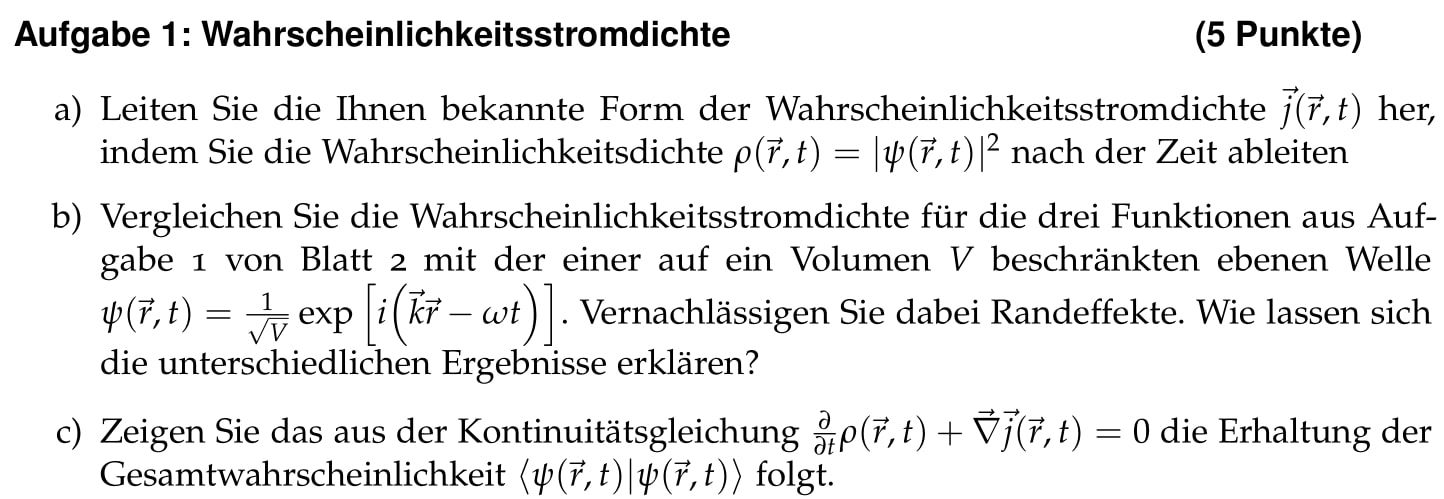
\includegraphics[width=0.75\textwidth]{./images/Aufgabe1.jpg}
    \label{fig:1}
\end{figure}

\subsection{a)}

    \begin{align*}
        \rho(\vec{r},t) &= \abs{\psi(\vec{r},t)}^2\\
        \frac{\partial\rho(\vec{r},t)}{\partial t} &= \frac{\partial}{\partial t} \abs{\psi(\vec{r},t)}^2\\
        &= \frac{\partial}{\partial t} (\psi^* \cdot \psi)\\
        &= \left( \psi^* \frac{\partial}{\partial t} \psi + \psi \frac{\partial}{\partial t} \psi^* \right)\\
        \frac{\partial \psi}{\partial t} &= \frac{1}{i\hbar} \left( -\frac{\hbar^2}{2m} \nabla^2 \psi + V\psi \right)\\
        &= - \frac{i\hbar}{2m}\nabla^2 \psi - \frac{i}{\hbar} V \psi\\
        \frac{\partial \psi^*}{\partial t} &= -\frac{i\hbar}{2m} \nabla^2 \psi^* + \frac{i}{\hbar} V \psi^*\\
        &= \psi^* \left( \frac{i\hbar}{2m} \nabla^2 \psi - \frac{i}{\hbar} V \psi \right) + \psi \left( -\frac{i\hbar}{2m} \nabla^2 \psi^* + \frac{i}{\hbar} V \psi^* \right)\\
        &= \frac{i\hbar}{2m} \psi^* \nabla^2 \psi \underbrace{\,-\,\frac{i}{\hbar} V \abs{\psi}^2}_{\text{Wegk\"urzen}} - \frac{i\hbar}{2m} \psi \nabla^2 \psi^* \underbrace{\,+\,\frac{i}{\hbar} V \abs{\psi}^2}_{\text{Wegk\"urzen}}\\
        &= - \nabla \underbrace{\left( \frac{\hbar}{2m} \left( \psi^* \nabla \psi - \psi \nabla \psi^* \right) \right)}_{\vec{j}} \tag{*}\\
        &= - \nabla \vec{j}\\
        \frac{\partial}{\partial t}\rho &= -\nabla\vec{j} 
    \end{align*}

\newpage
\subsection{b)}

    \flushleft{Die\;}\justifying folgenden Zustände werden dem Übungsblatt 2 entnommen:

    \noindent\makebox[\linewidth]{\rule{\textwidth}{1pt}}
    \begin{align*}
        \text{I} \qquad \psi_1 &= N_1 exp \left(-\frac{x^2}{2x_0^2} \right),\\
        \text{II} \qquad \psi_2 &= N_2 \frac{x}{x_0} exp \left( -\frac{x^2}{2x_0^2} \right),\\
        \text{III} \qquad \psi_3 &= N_3 \left( 2\frac{x^2}{x_0^2}-1 \right) exp \left( -\frac{x^2}{2x_0^2} \right)
    \end{align*}
    \noindent\makebox[\linewidth]{\rule{\textwidth}{1pt}}

    \begin{align*}
        \vec{j_1} &\stackrel{(*)}{=} \left( \frac{\hbar}{2m} \left( \psi_1^* \nabla \psi_1 - \psi_1 \nabla \psi_1^* \right) \right)\\
        &\nabla \psi_1 = N_1 exp \left(-\frac{x^2}{2x_0^2} \right)\\
        &= \frac{\hbar}{2mi} \left( N_1^2 exp \left( -\frac{x^2}{x_0^2} \right) \frac{-x}{x_0^2} - N_1^2 exp\left( -\frac{x^2}{x_0^2} \right) \frac{-x}{x_0^2} \right)\\
        &= 0\\
        \\
        \\
        \\
        \vec{j_2} &\stackrel{(*)}{=} \left( \frac{\hbar}{2m} \left( \psi_2^* \nabla \psi_2 - \psi_2 \nabla \psi_2^* \right) \right)\\
        &\text{\noindent\makebox[\linewidth]{\rule{\linewidth}{0.4pt}}}\\
        &\nabla \psi_2 = N_2 \left( \frac{1}{x_0^2} - \frac{x^2}{x_0^3} \right) exp \left( - \frac{x^2}{2x_0^2} \right)\\
        &\text{\noindent\makebox[\linewidth]{\rule{\linewidth}{0.4pt}}}\\
        &= \frac{\hbar}{2mi} \left( N_2^2 exp \left( -\frac{x^2}{x_0^2} \right) \left( \frac{1}{x_0} - \frac{x^2}{x_0^3} \right) - N_2^2 exp \left( -\frac{x^2}{x_0^2} \right) \left( \frac{1}{x_0} - \frac{x^2}{x_0^3} \right)  \right)\\
        &= 0\\
        \\
        \\
        \\
        \\
        \\
        \\
        \vec{j_3} &\stackrel{(*)}{=} \left( \frac{\hbar}{2m} \left( \psi_3^* \nabla \psi_3 - \psi_3 \nabla \psi_3^* \right) \right)\\
        &\text{\noindent\makebox[\linewidth]{\rule{\linewidth}{0.4pt}}}\\
        \nabla \psi_3 &= N_3 \nabla \left( \left( \frac{2x^2}{x_0^2} -1 \right) exp \left( -\frac{x^2}{2x_0^2} \right) \right)\\
        &= N_3 \left( \frac{4x}{x_0^2} + \left( \frac{2x^2}{x_0^2} - 1 \right) \left( -\frac{x}{x_0^2} \right) \right) exp \left( -\frac{x^2}{2x_0^2} \right)\\
        &= N_3 \left( \frac{5x}{x_0^2} - \frac{2x^3}{x_0^4} \right) exp \left( -\frac{x^2}{2x_0^2} \right)\\
        &\text{\noindent\makebox[\linewidth]{\rule{\linewidth}{0.4pt}}}\\
        &= \frac{\hbar}{2mi} \left( N_3^2 exp \left( -\frac{x^2}{x_0^2} \right) \left( \frac{5x}{x_0^2} - \frac{2x^3}{x_0^4} \right) - N_3^2 exp \left( -\frac{x^2}{x_0^2} \right) \left( \frac{5x}{x_0^2} - \frac{2x^3}{x_0^4} \right) \right)\\
        &= 0\\
        \\
        \\
        \\
        \Aboxed{\psi(\vec{r}, t) &= \frac{1}{\sqrt{V}} exp \left[ i \left( \vec{k} \vec{r} - \omega t \right) \right]}\\
        \vec{j} &\stackrel{(*)}{=} \left( \frac{\hbar}{2m} \left( \psi^* \nabla \psi - \psi \nabla \psi^* \right) \right)\\
        &\text{\noindent\makebox[\linewidth]{\rule{\linewidth}{0.4pt}}}\\
        \nabla \psi(\vec{r}, t) &= \frac{1}{\sqrt{V}} i\vec{k} exp \left[ i \left( \vec{k} \vec{r} - wt \right) \right]\\
        \nabla \psi^*(\vec{r}, t) &= \frac{1}{\sqrt{V}} (-i)\vec{k} exp \left[ -i \left( \vec{k} \vec{r} - wt \right) \right]\\
        &\text{\noindent\makebox[\linewidth]{\rule{\linewidth}{0.4pt}}}\\
        &= \frac{\hbar}{2mi} \left( \frac{1}{V^2} i\vec{k} - \frac{1}{V^2} (-i)\vec{k} \right)\\
        \vec{j} &= \frac{\hbar}{V^2} \vec{k}
    \end{align*}

\subsection{c)}

    \begin{align*}
        \frac{\partial}{\partial t} \rho &= -\nabla \vec{j}\\
        \frac{\partial}{\partial t} \abs{\psi}^2 &= - \nabla \vec{j}\\
        \frac{\partial}{\partial t} \int_{-\infty}^{\infty}  \abs{\psi}^2 \,\mathrm{d}x &= -\int_{-\infty}^{\infty}  \frac{\partial}{\partial x} \vec{j} \,\mathrm{d}x\\
        &= \vec{j}\, \vert_{-\infty}^{\infty}\\
        &\stackrel{(*)}{=} \left( \frac{\hbar}{2mi} \left( \psi^* \nabla \psi - \psi \nabla \psi^*   \right) \right) \big|_{-\infty}^{\infty}\\
        \frac{\partial}{\partial t} \int_{-\infty}^{\infty} \abs{\psi}^2 &= 0\\
        \frac{\partial}{\partial t} \langle \psi(\vec{r}, t) \vert \psi(\vec{r}, t) \rangle &= 0
    \end{align*}



\end{document}